%!TEX root = vorlage.tex

\section{Segmentation Pipeline}

Typically, semantic segmentation is done with a classifier which operates on
fixed-size feature inputs and a \textit{sliding-window}
approach~\cite{1467360,5490399,schroff2008object}. This means a classifier is
trained on images of a fixed size. The trained classifier is then fed with
rectangular regions of the image which are called \textit{windows}. Although
the classifier gets an image patch of e.g. $\SI{51}{\pixel} \times
\SI{51}{\pixel}$ of the environment, it might only classify the center pixel or
a subset of the complete window. This
segmentation pipeline is visualized in~\cref{fig:segmentation-pipeline}.

\begin{figure}
    \centering
    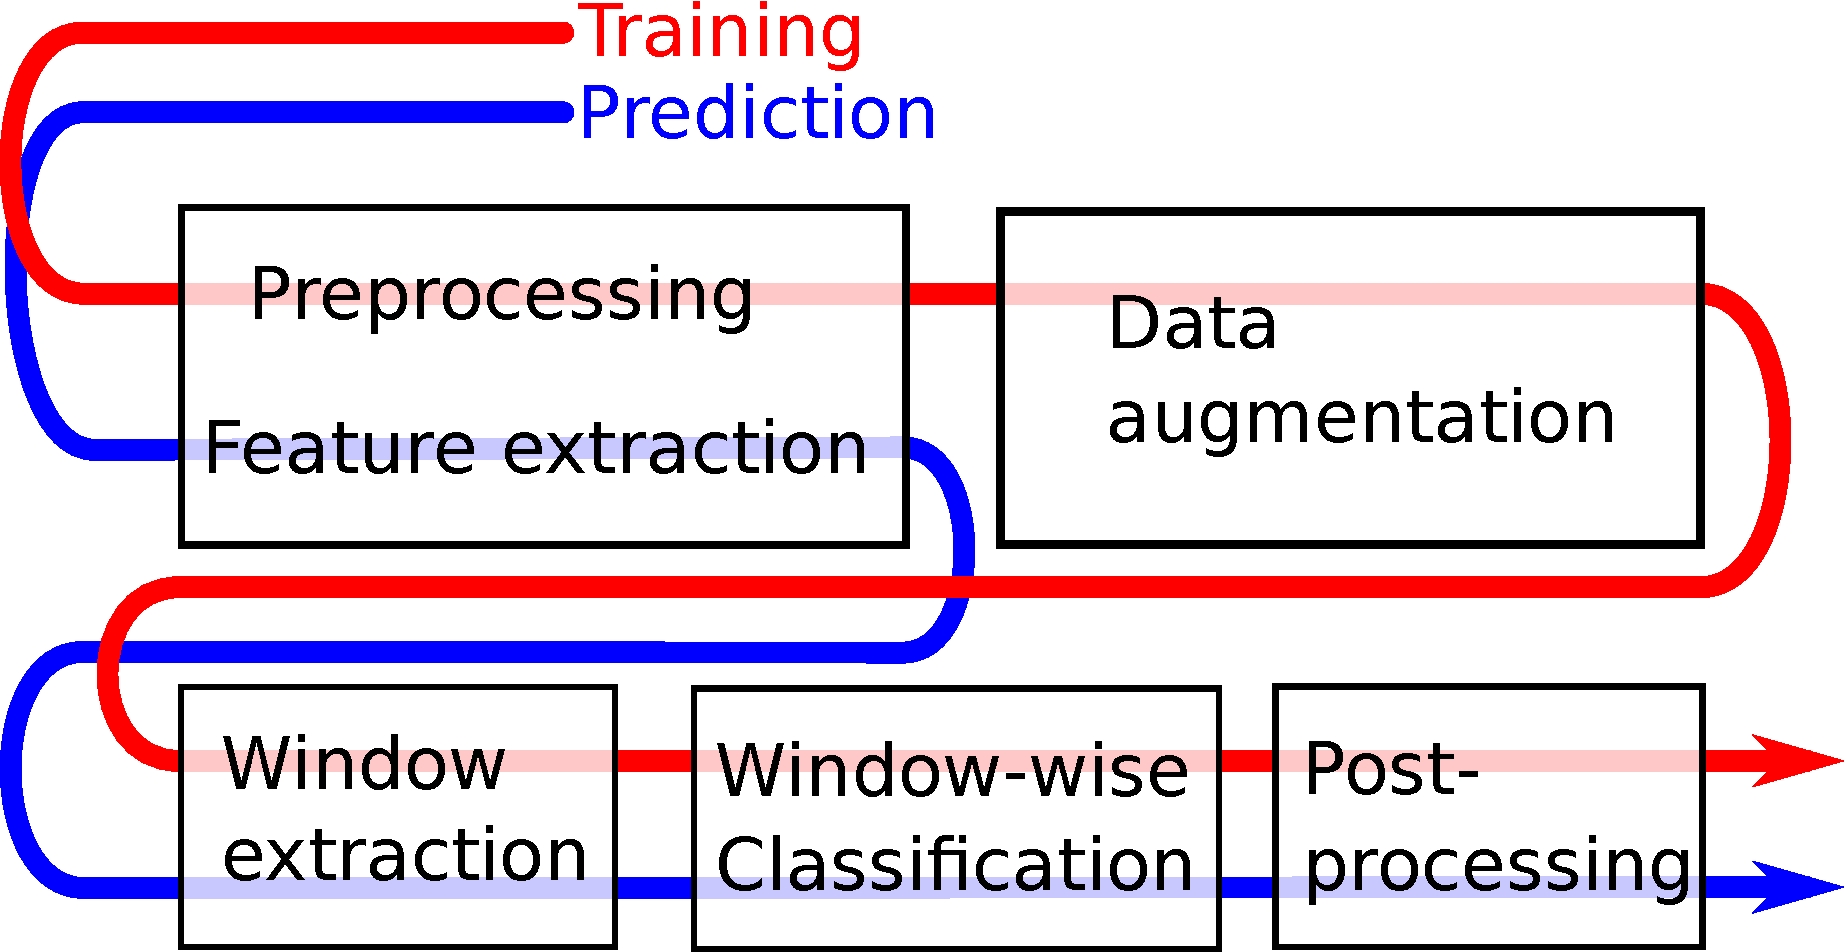
\includegraphics[width=\linewidth, keepaspectratio]{figures/segmentation-pipeline.pdf}
    \caption{A typical segmentation pipeline gets raw pixel data, applies
             preprocessing techniques like scaling and feature extraction like
             HOG features. For training, data augmentation techniques such as
             image rotation can be applied. For every single image, patches
             of the image called \textit{windows} are extracted and those
             windows are classified. The resulting semantic segmentation can
             be refined by simple morphologic operations or by more complex
             approaches such as \glspl{MRF}.}
    \label{fig:segmentation-pipeline}
\end{figure}

This approach was taken by~\cite{bittel2015pixel} and a majority of the VOC2007
participants~\cite{pascal-voc-2007}. As this approach has to apply the patch
classifier $512 \cdot 512 = \num{262144}$ times for images of size
$\SI{512}{\pixel} \times \SI{512}{\pixel}$, there are techniques for speeding
it up such as applying a stride and interpolating the results.

Neural networks are able to apply the sliding window approach in a very
efficient way by handling a trained network as a convolution and applying the
convolution on the complete image.

However, there are alternatives. Namely \glspl{MRF} and \glspl{CRF}
which take the information of the complete image and segment it in an holistic
approach.
